% !TEX root = ../thesis-example.tex
%
\chapter{Diseño Conceptual}
\label{sec:system}

\cleanchapterquote{La absoluta inspiración es la fecha límite.}{Nolan Bushnell}{(Fundador Atari, Inc.)}


\section{Necesidad}
\label{sec:system:sec1}

Los ejes de transmisión de las máquinas se encuentran sometidos constantemente a la fricción y a las vibraciones producto del contacto que existe entre estos y las piezas a las que estén conectados. Esto conlleva una serie de problemas como el aumento de la temperatura de operación y el desgaste de las piezas. Para disminuir estos efectos es necesaria la utilización de cojinetes o rodamientos sobre los que se sostengan y giren los ejes de transmisión.  

Algunas de estas máquinas requieren operar a un alto régimen de revoluciones, y para ello se han desarrollado los rodamientos magnéticos, los cuales generan un campo magnético que ayuda al eje de transmisión a permanecer en un estado de levitación, suprimiendo el contacto directo que tendría con un cojinete o rodamiento convencional y facilitando el giro del eje. Esto implica una disminución de la temperatura de operación, las vibraciones y el ruido, así como la posibilidad de reducir la potencia de los motores y los costos de mantenimiento relacionados al remplazo de piezas por desgaste y a la utilización de lubricantes. 

La mayoría de los rodamientos magnéticos desarrollados han sido de tipo activo, por lo que utilizan electroimánes para generar el campo magnético. El problema con esto es que requieren un constante suministro de energía eléctrica, lo que implica un incremento en el consumo de energía de la máquina en comparación con utilizar cojinetes convencionales. 

Es por ello que es necesario buscar una alternativa que pueda dar solución a este problema. El rodamiento magnético híbrido utiliza un imán permanente para generar un campo magnético base de levitación que mantendrá al eje en su posición una vez que los electroimánes lo hayan estabilizado, por lo que no requieren estar operando de forma permanente. 

\section{Especificaciones de Diseño del Producto (PDS)}
\label{sec:system:sec2}

Para delimitar los requerimientos de diseño se hace uso de una herramienta denominada PDS (por sus siglas en inglés Product Design Specifications). Esta herramienta documenta las características del producto y define las especificaciones y restricciones de diseño; dichas especificaciones permanecen en constante evolución a lo largo del proyecto, con base en la información adquirida a lo largo del desarrollo y las modificaciones que se consideren pertinentes.  
A continuación, se enlistan las especificaciones de diseño de los Rodamientos Magnéticos Híbridos:

\begin{itemize}
\addtolength{\itemsep}{-1mm}
\item Desarrollarse bajo una estructura lo más compacta posible sin sacrificar la funcionalidad.
\item Considerar el uso de materiales y componentes asequibles y con disponibilidad en el mercado. 
\item Capaz de soportar una carga estática de 1kg.
\item Considerar un diseño por módulos funcionales. 
\item Contar con un dispositivo mecánico de seguridad que sostenga el rotor en caso de que el sistema no se encuentre energizado.
\item Simplificación de las operaciones de ensamble. 
\item La levitación del rotor debe ser posible independientemente del material de fabricación de este. 
\end{itemize}



\section{Análisis Funcional}
\label{sec:system:sec3}

Una de las primeras consideraciones realizadas para el desarrollo del rodamiento magnético hibrido fue consolidar el diseño con base en módulos más sencillos que posteriormente pudieran integrarse para formar el sistema. Esta metodología es denominada Diseño Modular.
 
El diseño modular consiste en la creación de módulos funcionales, que unidos, forman estructuras mayores que pueden ser ensambladas de diferentes maneras o disposiciones; esta técnica tiene como finalidad que dichos módulos se puedan diseñar, desarrollar, probar y modificar de manera sencilla y lo más independientemente posible del resto del sistema. Esto simplifica en gran medida los procesos de manufactura y ensamble requeridos. 

Entre otras de sus ventajas podemos destacar:

\begin{itemize}[noitemsep]
\item Permite la planificación individual de los productos.
\item En caso de presentarse alguna falla, basta con determinar el módulo del que procede y realizar las reparaciones. 
\item Reduce los tiempos y costes de mantenimiento.
\end{itemize}

Con base en estos principios, se realizó la descomposición del rodamiento magnético híbrido en los siguientes módulos:

\begin{itemize}
%\begin{enumerate}[(a)]
\item Rodamiento magnético activo radial: genera el campo magnético para las cargas radiales por medio de electroimanes. 
\item Rodamiento magnético activo axial: genera el campo magnético para las cargas axiales por medio de electroimanes.
\item Arreglo de sensores de desplazamiento: miden la posición del rotor para realizar las correcciones necesarias para estabilizarlo. 
\item Módulo de compensación de cargas estáticas: provee un campo magnético base de levitación por medio de un imán permanente. 
\item Módulo de seguridad: consiste en un mecanismo que sea capaz de sostener y estabilizar el rotor cuando el sistema no se encuentre energizado, ya sea por acción del usuario o por un fallo en el suministro eléctrico. 
%\end{enumerate}
\end{itemize}

Cada uno de estos módulos cumple con una función específica, por lo que cuentan con características y requerimientos de operación particulares que hace posible que puedan diseñarse individualmente, pero al mismo tiempo son capaces de trabajar en conjunto y cumplir con la función principal del rodamiento magnético híbrido. 

Una vez que se ha determinado la división por módulos del sistema, se identifican las funciones o prestaciones que debe cumplir para cubrir la necesidad, y convertirlas en especificaciones de diseño.

A continuación se muestra el diagrama por áreas funcionales del rodamiento magnético híbrido, donde se aprecia cómo interactúan los módulos con el resto de los subsistemas:

\begin{figure}[htb]
\centering
	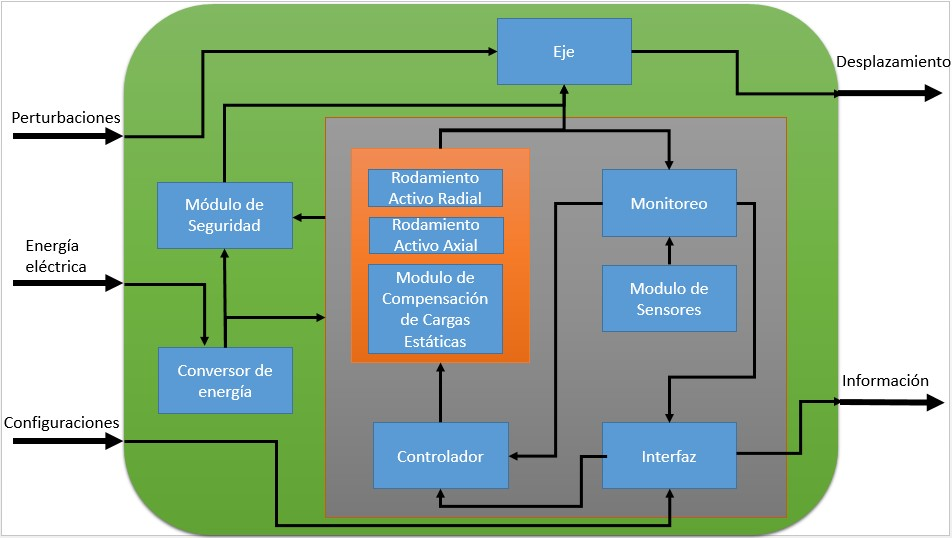
\includegraphics[width=\textwidth]{images/Capitulo_2/DiagramaFuncional}
	\caption{\textit{Diagrama Funcional.}}
	\label{fig:system:example1}
\end{figure}

Del diagrama de áreas funcionales podemos reconocer que el sistema cuenta con 2 entradas que determinan el funcionamiento y el comportamiento del mismo: el suministro de energía eléctrica y las perturbaciones que llegan al sistema. Este diagrama se divide en 3 secciones principales: la primera sección lo componen los módulos que generan los campos magnéticos de levitación, los cuales deben variar de acuerdo a lo que indique el controlador. Este se encuentra dominado por el monitoreo del módulo de sensores y la interfaz de usuario, la cual además muestra información sobre la posición del rotor. 

La tercera sección incluye el convertidor de energía que alimenta todos los sistemas eléctricos, incluyendo el módulo de seguridad, el cual se rige a través de la información que provea el controlador, ya que este sólo actúa con el corte del suministro eléctrico o por alguna falla detectada por el controlador. 


\section{Diseño Conceptual del Producto}
\label{sec:system:sec4}

La arquitectura del sistema fue planteada con base en la investigación teórica sobre las características generales de los rodamientos magnéticos y en la división por módulos funcionales, de manera que pudieran diseñarse individualmente. 

\subsection{Rodamiento Magnético Activo Radial}

Los rodamientos magnéticos activos utilizan un arreglo de electroimanes opuestos para generar los campos magnéticos de levitación, y están diseñados para soportar las cargas radiales que actúan sobre el rotor, manteniéndolo centrado sobre el eje de rotación de la máquina.

\begin{figure}[htb]
\centering
	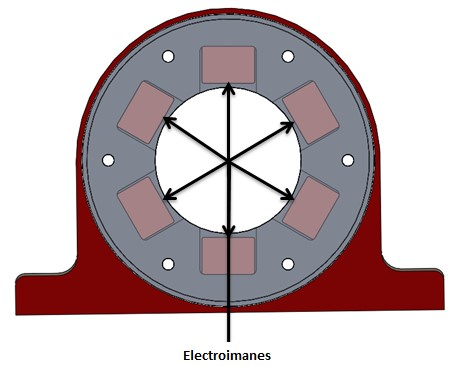
\includegraphics[scale=.65]{images/Capitulo_2/RMAR}
	\caption{\textit{Diseño conceptual del rodamiento magnético activo radial.}}
	\label{fig:system:example1}
\end{figure}

\subsection{Rodamiento Magnético Activo Axial}

Como su nombre lo dice, los rodamientos magnéticos axiales están diseñados para soportar cargas axiales. Estos utilizan un collar de soporte, el cual consiste por lo general en un disco plano, sólido, de material ferromagnético fijado al rotor. Los electroimánes en forma de disco están situados a cada lado del collar y sujetos a la carcasa de la máquina. Utilizan un sensor o arreglo de sensores que mide la posición del rotor en dirección axial. 

\begin{figure}[htb]
\centering
	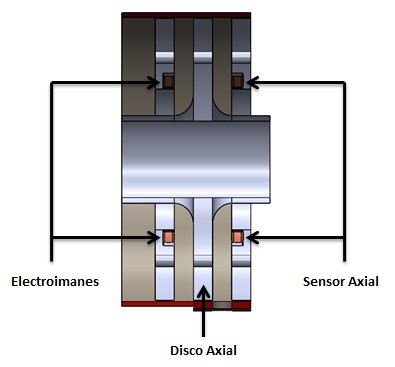
\includegraphics[scale=.65]{images/Capitulo_2/RMAA}
	\caption{\textit{Diseño conceptual del rodamiento magnético activo axial.}}
	\label{fig:system:example1}
\end{figure}

\subsection{Módulo de Sensores}

Este arreglo de sensores para el rodamiento magnético activo radial 
envía las señales de posición del rotor al controlador. El controlador utiliza esta información para modificar el campo electromagnético en el rodamiento.

\begin{figure}[htb]
\centering
	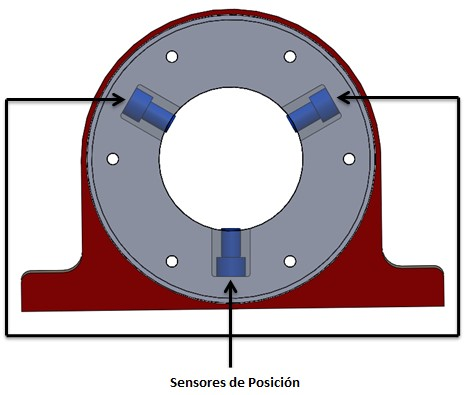
\includegraphics[scale=.65]{images/Capitulo_2/MS}
	\caption{\textit{Diseño conceptual del arreglo de sensores para los desplazamientos radiales.}}
	\label{fig:system:example1}
\end{figure}

%\clearpage

\subsection{Módulo de Compensación de Cargas Estáticas}

Este módulo se basa en el principio de funcionamiento de los rodamientos magnéticos pasivos. Utiliza un imán permanente para generar un campo magnético base de levitación que ayude a disminuir el consumo de energía del rodamiento magnético radial. Debe utilizar un mecanismo de desplazamiento que varíe la distancia entre el imán permanente y el rotor para ajustar el campo magnético. 

\begin{figure}[htb]
\centering
	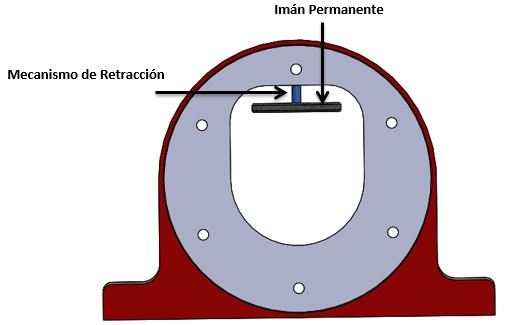
\includegraphics[scale=.70]{images/Capitulo_2/MCCE}
	\caption{\textit{Diseño Conceptual del módulo de compensación para cargas estáticas.}}
	\label{fig:system:example1}
\end{figure}

\subsection{Módulo de Seguridad}

Uno de los elementos más importantes con los que debe contar un rodamiento magnético es un mecanismo auxiliar que tenga como finalidad soportar el rotor en caso de un corte en la energía. El rotor no debe de hacer contacto con el mecanismo auxiliar durante el funcionamiento normal de la máquina.

\begin{figure}[htb]
\centering
	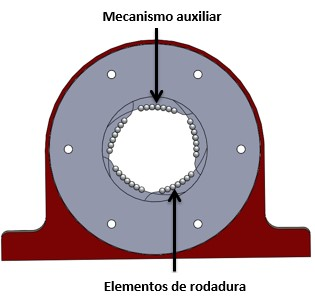
\includegraphics[scale=.90]{images/Capitulo_2/MSG}
	\caption{\textit{Diseño conceptual del dispositivo auxiliar para el módulo de seguridad.}}
	\label{fig:system:example1}
\end{figure}

\subsection{Collarín de Levitación}

Con el propósito de lograr la levitación del rotor sin importar el material del que esté fabricado, se propone el uso de un collarín de material ferromagnético que contenga al eje del rotor dentro del rodamiento. 

\begin{figure}[htb]
\centering
	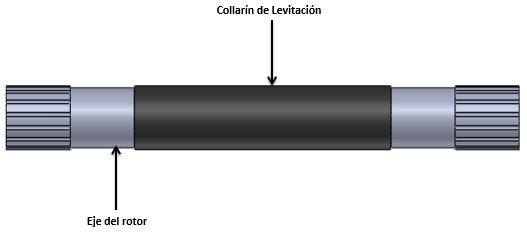
\includegraphics[scale=.90]{images/Capitulo_2/CL}
	\caption{\textit{Diseño Conceptual del collarín de levitación.}}
	\label{fig:system:example1}
\end{figure}

\subsection{Rodamiento Magnético Híbrido: Integración de los Módulos}

Aunque cada uno de los módulos es diseñado individualmente, están contemplados para funcionar de manera conjunta y ser ensamblados dentro del mismo armazón. La integración de todos los módulos nos daría como resultado el Rodamiento Magnético Híbrido. 

\begin{figure}[htb]
\centering
	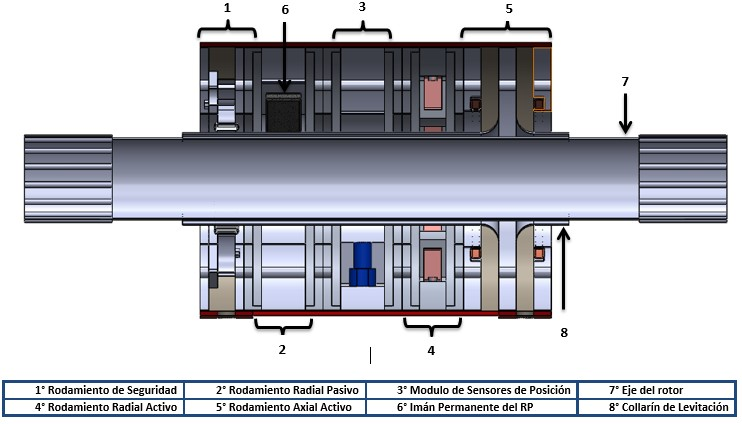
\includegraphics[width=\textwidth]{images/Capitulo_2/RMH}
	\caption{\textit{Diseño Conceptual del Rodamiento Magnético Híbrido.}}
	\label{fig:system:example1}
\end{figure}
